\documentclass{beamer}
\usepackage{pgfplots}
\pgfplotsset{compat=1.18}
\begin{document}
\begin{frame}{only}
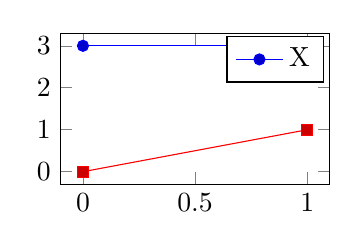
\begin{tikzpicture}
\begin{axis}[width=5cm, height=3.5cm]
\only<2>{\addplot coordinates {(0,3) (1,3)};}
\addplot coordinates {(0,0) (1,1)};
\only<2>{\addlegendentry{X}}
\end{axis}
\end{tikzpicture}
\end{frame}
\begin{frame}{uncover}
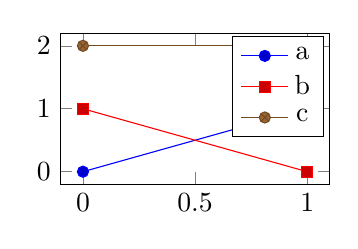
\begin{tikzpicture}
\begin{axis}[width=5cm, height=3.5cm]
\addplot coordinates {(0,0) (1,1)};
\uncover<2>{\addplot coordinates {(0,1) (1,0)};}
\visible<2>{\addplot coordinates {(0,2) (1,2)};}
\legend{a,b,c}
\end{axis}
\end{tikzpicture}
\end{frame}
\begin{frame}{alt}
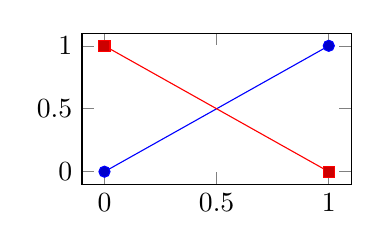
\begin{tikzpicture}
\begin{axis}[width=5cm, height=3.5cm]
\alt<2>{\addplot coordinates {(0,0) (1,1)};}{\addplot coordinates {(0,1) (1,0)};}
\end{axis}
\end{tikzpicture}
\end{frame}
\begin{frame}{onslide}
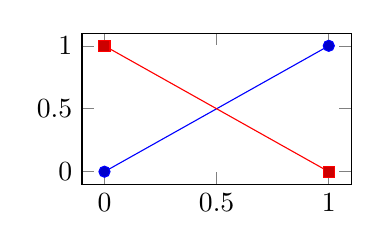
\begin{tikzpicture}
\begin{axis}[width=5cm, height=3.5cm]
\addplot coordinates {(0,0) (1,1)};
\onslide<2->
\addplot coordinates {(0,1) (1,0)};
\end{axis}
\end{tikzpicture}
\end{frame}
\begin{frame}{draw in axis}
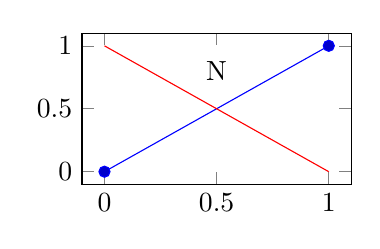
\begin{tikzpicture}
\begin{axis}[width=5cm, height=3.5cm]
\addplot coordinates {(0,0) (1,1)};
\only<2>{\draw[red] (axis cs:0,1) -- (axis cs:1,0);}
\uncover<2>{\node at (axis cs:0.5,0.8) {N};}
\end{axis}
\end{tikzpicture}
\end{frame}
\end{document}
